% Options for packages loaded elsewhere
\PassOptionsToPackage{unicode}{hyperref}
\PassOptionsToPackage{hyphens}{url}
\PassOptionsToPackage{dvipsnames,svgnames,x11names}{xcolor}
%
\documentclass[
  number]{elsarticle}

\usepackage{amsmath,amssymb}
\usepackage{iftex}
\ifPDFTeX
  \usepackage[T1]{fontenc}
  \usepackage[utf8]{inputenc}
  \usepackage{textcomp} % provide euro and other symbols
\else % if luatex or xetex
  \usepackage{unicode-math}
  \defaultfontfeatures{Scale=MatchLowercase}
  \defaultfontfeatures[\rmfamily]{Ligatures=TeX,Scale=1}
\fi
\usepackage{lmodern}
\ifPDFTeX\else  
    % xetex/luatex font selection
\fi
% Use upquote if available, for straight quotes in verbatim environments
\IfFileExists{upquote.sty}{\usepackage{upquote}}{}
\IfFileExists{microtype.sty}{% use microtype if available
  \usepackage[]{microtype}
  \UseMicrotypeSet[protrusion]{basicmath} % disable protrusion for tt fonts
}{}
\makeatletter
\@ifundefined{KOMAClassName}{% if non-KOMA class
  \IfFileExists{parskip.sty}{%
    \usepackage{parskip}
  }{% else
    \setlength{\parindent}{0pt}
    \setlength{\parskip}{6pt plus 2pt minus 1pt}}
}{% if KOMA class
  \KOMAoptions{parskip=half}}
\makeatother
\usepackage{xcolor}
\setlength{\emergencystretch}{3em} % prevent overfull lines
\setcounter{secnumdepth}{5}
% Make \paragraph and \subparagraph free-standing
\makeatletter
\ifx\paragraph\undefined\else
  \let\oldparagraph\paragraph
  \renewcommand{\paragraph}{
    \@ifstar
      \xxxParagraphStar
      \xxxParagraphNoStar
  }
  \newcommand{\xxxParagraphStar}[1]{\oldparagraph*{#1}\mbox{}}
  \newcommand{\xxxParagraphNoStar}[1]{\oldparagraph{#1}\mbox{}}
\fi
\ifx\subparagraph\undefined\else
  \let\oldsubparagraph\subparagraph
  \renewcommand{\subparagraph}{
    \@ifstar
      \xxxSubParagraphStar
      \xxxSubParagraphNoStar
  }
  \newcommand{\xxxSubParagraphStar}[1]{\oldsubparagraph*{#1}\mbox{}}
  \newcommand{\xxxSubParagraphNoStar}[1]{\oldsubparagraph{#1}\mbox{}}
\fi
\makeatother


\providecommand{\tightlist}{%
  \setlength{\itemsep}{0pt}\setlength{\parskip}{0pt}}\usepackage{longtable,booktabs,array}
\usepackage{calc} % for calculating minipage widths
% Correct order of tables after \paragraph or \subparagraph
\usepackage{etoolbox}
\makeatletter
\patchcmd\longtable{\par}{\if@noskipsec\mbox{}\fi\par}{}{}
\makeatother
% Allow footnotes in longtable head/foot
\IfFileExists{footnotehyper.sty}{\usepackage{footnotehyper}}{\usepackage{footnote}}
\makesavenoteenv{longtable}
\usepackage{graphicx}
\makeatletter
\newsavebox\pandoc@box
\newcommand*\pandocbounded[1]{% scales image to fit in text height/width
  \sbox\pandoc@box{#1}%
  \Gscale@div\@tempa{\textheight}{\dimexpr\ht\pandoc@box+\dp\pandoc@box\relax}%
  \Gscale@div\@tempb{\linewidth}{\wd\pandoc@box}%
  \ifdim\@tempb\p@<\@tempa\p@\let\@tempa\@tempb\fi% select the smaller of both
  \ifdim\@tempa\p@<\p@\scalebox{\@tempa}{\usebox\pandoc@box}%
  \else\usebox{\pandoc@box}%
  \fi%
}
% Set default figure placement to htbp
\def\fps@figure{htbp}
\makeatother

\usepackage{booktabs}
\usepackage{caption}
\usepackage{longtable}
\usepackage{colortbl}
\usepackage{array}
\usepackage{anyfontsize}
\usepackage{multirow}
\makeatletter
\@ifpackageloaded{float}{}{\usepackage{float}}
\floatstyle{plain}
\@ifundefined{c@chapter}{\newfloat{suppfig}{h}{losuppfig}}{\newfloat{suppfig}{h}{losuppfig}[chapter]}
\floatname{suppfig}{Figure S}
\newcommand*\quartosuppfigref[1]{Figure \hyperref[#1]{S\ref{#1}}}
\@ifpackageloaded{caption}{}{\usepackage{caption}}
\DeclareCaptionLabelFormat{quartosuppfigreflabelformat}{#1#2}
\captionsetup[suppfig]{labelformat=quartosuppfigreflabelformat}
\newcommand*\listofsuppfigs{\listof{suppfig}{List of Supplementary Figures}}
\makeatother
\makeatletter
\@ifpackageloaded{float}{}{\usepackage{float}}
\floatstyle{plain}
\@ifundefined{c@chapter}{\newfloat{supptab}{h}{losupptab}}{\newfloat{supptab}{h}{losupptab}[chapter]}
\floatname{supptab}{Table S}
\newcommand*\quartosupptabref[1]{Table \hyperref[#1]{S\ref{#1}}}
\@ifpackageloaded{caption}{}{\usepackage{caption}}
\DeclareCaptionLabelFormat{quartosupptabreflabelformat}{#1#2}
\captionsetup[supptab]{labelformat=quartosupptabreflabelformat}
\newcommand*\listofsupptabs{\listof{supptab}{List of Supplementary Tables}}
\makeatother
\makeatletter
\@ifpackageloaded{caption}{}{\usepackage{caption}}
\AtBeginDocument{%
\ifdefined\contentsname
  \renewcommand*\contentsname{Table of contents}
\else
  \newcommand\contentsname{Table of contents}
\fi
\ifdefined\listfigurename
  \renewcommand*\listfigurename{List of Figures}
\else
  \newcommand\listfigurename{List of Figures}
\fi
\ifdefined\listtablename
  \renewcommand*\listtablename{List of Tables}
\else
  \newcommand\listtablename{List of Tables}
\fi
\ifdefined\figurename
  \renewcommand*\figurename{Figure}
\else
  \newcommand\figurename{Figure}
\fi
\ifdefined\tablename
  \renewcommand*\tablename{Table}
\else
  \newcommand\tablename{Table}
\fi
}
\@ifpackageloaded{float}{}{\usepackage{float}}
\floatstyle{ruled}
\@ifundefined{c@chapter}{\newfloat{codelisting}{h}{lop}}{\newfloat{codelisting}{h}{lop}[chapter]}
\floatname{codelisting}{Listing}
\newcommand*\listoflistings{\listof{codelisting}{List of Listings}}
\makeatother
\makeatletter
\makeatother
\makeatletter
\@ifpackageloaded{caption}{}{\usepackage{caption}}
\@ifpackageloaded{subcaption}{}{\usepackage{subcaption}}
\makeatother

\usepackage[]{natbib}
\bibliographystyle{elsarticle-num}
\usepackage{bookmark}

\IfFileExists{xurl.sty}{\usepackage{xurl}}{} % add URL line breaks if available
\urlstyle{same} % disable monospaced font for URLs
\hypersetup{
  pdftitle={Investigating the Spatial Variability in Soil Geochemical and Colour Properties Across Two Contrasting Land Uses},
  pdfauthor={Maria Luna Miño; Alexander J Koiter; Taras E Lychuk; Arnie Waddel; Alan Moulin},
  pdfkeywords={Soil geochemistry, Soil colour, Spatial analysis},
  colorlinks=true,
  linkcolor={blue},
  filecolor={Maroon},
  citecolor={Blue},
  urlcolor={Blue},
  pdfcreator={LaTeX via pandoc}}


\setlength{\parindent}{6pt}
\begin{document}

\begin{frontmatter}
\title{Investigating the Spatial Variability in Soil Geochemical and
Colour Properties Across Two Contrasting Land Uses}
\author[1]{Maria Luna Miño%
%
}
 \ead{LUNAMIMA56@brandonu.ca} 
\author[2]{Alexander J Koiter%
\corref{cor1}%
}
 \ead{koitera@brandonu.ca} 
\author[3]{Taras E Lychuk%
%
}
 \ead{taras.lychuk@AGR.GC.CA} 
\author[3]{Arnie Waddel%
%
}
 \ead{arnie.waddell@AGR.GC.CA} 
\author[3]{Alan Moulin%
%
}
 \ead{apmaafc7788@gmail.com} 

\affiliation[1]{organization={Brandon University, Masters in
Environmental and Life Sciences},addressline={270 18th
St},city={Brandon},postcode={R7A 6A9},postcodesep={}}
\affiliation[2]{organization={Brandon University, Department of
Geography and Environment},addressline={270 18th
St},city={Brandon},postcode={R7A 6A9},postcodesep={}}
\affiliation[3]{organization={Agriculture and Agri-Food Canada, Brandon
Research and Development Centre},addressline={2701 Grand Valley
Road},city={Brandon},postcode={R7A 5Y3},postcodesep={}}

\cortext[cor1]{Corresponding author}





        
\begin{abstract}
Quantification and accurate assessment of the spatial variability and
distribution of soil physical and biogeochemical properties are vital
components of agri-environmental research and modeling, including
sediment source fingerprinting. Understanding the distribution of soil
properties is crucial in the development of appropriate, reliable, and
efficient sampling campaigns. This study was aimed to investigate the
spatial variability in soil geochemical and colour (i.e., spectral
reflectance) soil properties (\textless63um) across two contrasting land
uses. The main objectives of this study are to: 1) quantify the spatial
variability of geochemical and colour properties at a field-scale
(\textasciitilde{} 40 ha) across agricultural and forested sites; 2)
evaluate the spatial variability and distribution of soil properties and
its relation to seven terrain attributes (e.g., catchment area,
elevation). A combination of univariate analysis and geostatistical
methods were applied to characterize the soil geochemistry and colour
properties. This information was used to both quantify and assess the
variability in soil properties. The variability and spatial
autocorrelation were generally both site and soil property specific. For
a selection of soil properties exhibiting some spatial autocorrelation,
random forest regression was used to indentify the relative importance
of terrain attributes on observed patterns of soil geochemical and
colour properties. Elevation was found to explain the greatest amount of
the variation in soil properties followed by the SAGA wetness index and
relative slope position. These types of information can be used to help
create efficient soil sampling designs by providing information that can
inform sampling locations and number of samples collected in order to
meet research needs and objectives.
\end{abstract}





\begin{keyword}
    Soil geochemistry \sep Soil colour \sep 
    Spatial analysis
\end{keyword}
\end{frontmatter}
    

\section{Introduction}\label{introduction}

Variation in soil biological, chemical, and physical properties occurs
across the landscape and in response to both regional and local (i.e.,
field-scale) variations in the five soil forming factors: parent
material, relief or topography, biota, climate, and time. Superimposed
on this is the influence of changes in land use and current and historic
management practices which can further modify soil properties.
Quantifying and understanding the patterns and drivers for this
variation is an important component of many agri-environmental studies.
For example, to meet the desired level of precision for agronomic and
environmental nutrient management plans the spatial variability in soil
nutrients will influence the soil sampling design in terms of number and
locations of soil samples \citep{starr1995, kariuki2009}.

Sediment source fingerprinting is a watershed-scale technique that is
used to identify and quantify the relative proportions of sediment
derived from unique sources. This technique uses natural occurring
biogeochemical properties as fingerprints (i.e., tracers) to
discriminate between potential sources of sediment and are linked to
downstream sediment using mixing models. From a sediment fingerprinting
perspective, investigating the spatial variability of soil properties at
a watershed-scale can be advantageous to identify, classify, and
distinguish between potential sources of sediment \citep{pulley2017}.
However, investigating spatial variability at smaller scales is less
common \citep[e.g.,][]{du2017, pulley2018, collins2019, lunamiño2024}
and remains a research priority \citep{collins2020}.

There are three main, interconnected, ways that spatial variability in
fingerprint properties are an important aspect of sediment
fingerprinting. First is to adequately quantify the fingerprint
properties such that it is representative of that source. For some
fingerprints the variability is not random but rather varies in a more
systematic way. For example, the pattern of fallout radionuclides will
reflect the patterns of soil erosion and deposition
\citep{wilkinson2015}. Designing and implementing source sampling plans
need to take this into consideration as the sampling designed used has
been shown to influence the characterization of wide range of commonly
used fingerprints \citep{lunamiño2024}.

Secondly, the issue of spatial variability of fingerprint properties is
further complicated by overlying spatial variability in the rates of
erosion and sediment delivery. Incorporation of both types of
variability into the mixing model will provide a more reliable estimate
of the proportion of sediment derived from each source. Many mixing
models have well defined inputs (sources) and outputs (sediment) that
are characterized by their mean and standard deviation and the spatial
distribution or pattern of fingerprints are not considered. This is not
ideal as the values of samples that are collected closer, and more
hydrologically connected, to the stream network may in fact a better
representation of that source despite potentially deviating from the
mean value. This issue can be addressed by strategic sampling where the
more likely to erode areas are targeted for sampling. However, a
considerable amount of information and insight is lost through that
approach. There has been some progress using information on erosion
rates to calculate a erosion rate-weighted mean
\citep{wilkinson2015, du2017} and using spatially interpolated maps of
fingerprint values to provided a finer resolution of the fingerprint
variability within each source \citep{haddadchi2019}.

Secondly, understanding the geomorphic, hydrologic, and biochemical
processes that have led to the observed patterns in spatial variability
helps in the selection of robust and reliable fingerprints and/or guide
the sampling design for source characterization. In selecting
fingerprints that provide good discrimination between sources many
studies typically used a statistical-based approach \citep{collins1997}.
However, there are concerns that this approach may result in the
inclusion of false positives (i.e., type I error) or non-conservative
fingerprints \citep{koiter2013}. Consequently, there has been a call for
the inclusion of a process-based (e.g., weathering, erosion) or
geologic/lithologic-based explanation of the fingerprints selected to
address these concerns \citep{collins2020}. Furthermore, there is also a
lack of standardization in how sediment source areas are sampled (e.g.,
judgement, random, transect, grid, stratified) and it can be difficult
to have an efficient sampling design without prior knowledge of why and
how soil properties vary across the landscape \citep{lunamiño2024}.
Prior knowledge of the spatial variability of soil fingerprint
properties would be beneficial; however, in practice this can be
difficult, particularly with geochemical properties as routine lab
analysis often return information on more than 50 elements. The spatial
patterns of some soil properties are well studied because of their
agronomic importance or ability to infer other important soil properties
and processes and can include fallout radionuclides {[}e.g.,
\textsuperscript{137}Cs, \textsuperscript{7}Be; \citep{ritchie1970}{]},
plant nutrients {[}e.g., N, P; \citep{vasu2017}{]}, soil colour {[}e.g.,
hue, value; \citep{viscarrarossel2006}{]}, major non-acid forming
cations {[}e.g., Ca, Na; \citep{sun2021}{]}. In contrast, other soil
properties including rare Earth elements and trace metals the processes
leading to their distribution across the landscape is less studied or it
is difficult to make generalizations (i.e., site specific).

Terrain attributes such as elevation, slope curvature, slope position,
and soil wetness have been shown to be useful information in the
understanding and modelling of a range of soil properties including soil
moisture \citep{beaudette2013}, texture \citep{kokulan2018}, colour
\citep{brown2004}, organic matter \citep{zhang2012}, conductivity
\citep{umali2012}, and geochemistry \citep{lima2023}. Similar techniques
may provide additional insight into the pedologic and geomorphic
processes that drive the observed patterns of fingerprint properties
within a given source. This information can be used to guide sampling
design and interpret the data it provides.

This study builds on the previous work of Luna Miño \citep{lunamiño2024}
where the impact of three different sampling designs on the
characterization of source materials, within the framework of the
sediment fingerprinting approach, was assessed. This study expands that
study by using the data from grid sampling approach to assess the
spatial autocorrelation, create iso-fingerprint maps, and identify
important terrain attributes driving the observed patterns. The
objectives of this study were (1) to investigate the spatial variability
of a range of soil colour and geochemical properties in an agricultural
and forested site; and (2) to assess the relative importance and
correlation of terrain attributes with the spatial distribution of these
soil properties.

\section{Methods}\label{methods}

\subsection{Site description}\label{site-description}

Two sites of contrasting land uses located in the Wilson Creek Watershed
(WCW), near McCreary, Manitoba, Canada were selected to investigate the
spatial variability in fingerprint properties. The headwaters of the WCW
are located on top of the Manitoba Escarpment within the boundary of
Riding Mountain National Park. There is a \textasciitilde300m drop in
elevation crosses the escarpment where the streams become deeply
incised. At the base of the escarpment is a large alluvial fan situated
in the lacustrine deposits of glacial lake Aggasiz where the main stem
has a meandering form. However, beyond the national park boundary the
stream flows straight through an engineered drain until it reaches the
Turtle river (Figure~\ref{fig-location_map}). Both sites are both
hydrologicaly connected to the mainstem of the Wilson Creek

The first site was a mixedwood forest including white and black spruce
(Picea glauca, Picea mariana), balsam fir (Abies balsamea), larch (Larix
laricina) and young stands of deciduous trees including trembling aspen
(Populus tremuloides). The forested site is located within the
boundaries of the national park where there is little disturbance beyond
recreational hiking trails. The soil within the park are not well mapped
but likely are part of the Grey Wooded soil association (Luvisol)
consisting of fine sandy loam to clay loam soils developed on boulder
till of mostly shale with some limestone, and granitic rocks
\citep{ehrlich1958}. The second site is under agricultural production
and includes rotations of grain crops and forage. The site is mapped to
the Edwards Soil Series (Cumulic Regosol) consisting of silty clay loam
to silty clay soil developed on recent alluvial deposits
\citep{ehrlich1958}.

The Köppen-Geiger climate classification of the WCW is cold, without dry
season, and with warm summer (Dfb) \citep{beck2018}. The average annual
precipitation is \textasciitilde539 mm, with approximately 27\% falling
as snow with a mean annual temperature is 3.0°C
\citep{environmentandclimatechangecanada2024}. The hydrology of the
watershed is snowmelt dominated with \textasciitilde{} 80\% of the
cumulative runoff occurring during the spring season (May and June)
\citep{mackay1970}.

\begin{figure}[H]

\centering{

\pandocbounded{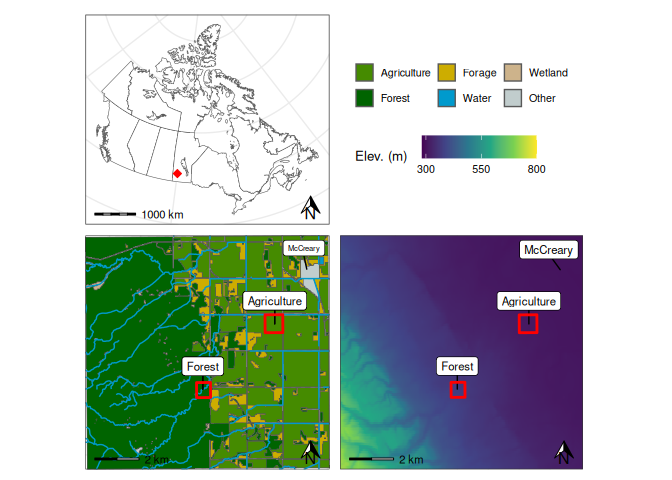
\includegraphics[keepaspectratio]{index_files/figure-latex/notebooks-location_map-fig-location_map-output-2.png}}

}

\caption{\label{fig-location_map}Map showing the location of the study
sites within Canada, and the regional land use and topography.}

\end{figure}%

\textsubscript{Source:
\href{https://alex-koiter.github.io/spatial-variability-soil-manuscript/notebooks/location_map.qmd.html\#cell-fig-location_map}{Research
Site Locations}}

\subsection{Soil sampling and
analysis}\label{soil-sampling-and-analysis}

This study uses samples and data collected as part of the grid sampling
design outlined in Luna Miño \citep{lunamiño2024}. Briefly, at each site
49 samples were collected using a soil auger on a 7x7 grid at a 100m
spacing. Within the forested surface soil samples were collected below
the LFH layer to a depth of 5cm, and the agricultural site was sampled
to a depth of 15cm to account for the regular mixing of the soil due to
tillage and other field operations.

Samples were dried, homogenized with a motar and pestle, and sieved
through a 63 𝜇m sieve to remove the sand fraction. The sand fraction was
removed in an effort to reduce the differences in grain size and organic
matter content between the two sites \citep{laceby2017}. Samples were
analyzed for a broad suite geochemical element using inductively coupled
plasma mass spectrometry (ICP-MS) following a microwave-assisted
digestion with aqua-regia (ALS Mineral Division, North Vancouver, BC,
Canada). Spectral measurements were made with a spectroradiometer (ASD
FieldSpecPro Malvern Panalytical Inc Westborough MA 01581, United
States). Spectral reflectance measurements were taken in 1 nm increments
over the 0.4-2.5 μm wavelength range. Both samples and Spectralon
standard (white reference) were illuminated with a white light source
using a halogen-based lamp (12 VDC, 20 Watt). Following the method
outlined in Boudreault et al. \citep{boudreault2018}, fifteen colour
coefficients (R, G, B, x, y, Y, X, Z, L, a*, b*, u*, v*, c*, h*) were
calculated for each sample \citep{koiter2021}. Based on the results of
Luna Miño \citep{lunamiño2024}, a composite fingerprint consisting of 10
geochemical elements (Ca, Co, Cs, Fe, Li, La, Nb, Ni, Rb, and Sr) and
five colour coefficients (a, b, c, h, and x) were identifying as
providing a strong discrimination between the agricultural and forested
surface soils. These fifteen soil properties are the focus of the
detailed spatial analysis detailed in this study.

\subsection{Geospatial and terrain
analysis}\label{geospatial-and-terrain-analysis}

All geostatistics were performed with ArcGIS Pro \citep[v
3.3.0][]{esri2024}. Semivariograms were used to quantify spatial
correlation for each of the 15 soil properties. The optimization tool,
based on minimizing the mean square error, was used to parameterize the
semivariogram model. Kriging was used to interpolate and generate maps
of each soil property. The exploratory interpolation tool
(Geostatistical Analyst extension) was used to select the kriging type
with the highest ranked prediction accuracy.

A Digital Elevation Model (DEM) for the forested site was acquired from
publicly available data \citep{naturalresourcescanada2024}. A DEM for
the agricultural site was generated by photogrammetry using UAV imagery,
including the use of ground control and check points, with Agisoft
Metashape Professional \citep[v1.8.2][]{agisoft2021}. Ordinary kriging
was used to calculate a 1 m gridded digital elevation model for each
site. Geographic information software \citep[SAGA v2.1.4][]{conrad2015}
was used to calculate six additional terrain attributes and included
plan and profile curvatures, saga wetness index, catchment area,
relative slope position, vertical channel network distance.

\subsection{Data analysis}\label{data-analysis}

All subsequent statistical analysis was undertaken using R statistical
Software v4.4.0 \citep{rcoreteam2024} through RStudio Integrated
Development Environment v2024.04.2 \citep{rstudio2024}. Plots and maps
were created using the R package \texttt{ggplot2} v 3.5.1
\citep{wickham2016}. Skewness was categorized as values between -0.5 and
0.5 considered approximately symmetric, -1.0 to -0.5 or 0.5 to 1 as
moderately skewed, and \textless{} -1.0 or \textgreater{} 1.0 as highly
skewed. Coefficient of variation (CV) thresholds were categorized as low
(\textless15\%), moderate (15--35\%), high (35--75\%), and very high
(\textgreater75\%) .Interpolated soil property and terrain attribute
data were resampled to a 10 m resolution prior to analysis
\citep[\texttt{terra} v1.8.29][]{hijmans2024}. Random Forest Regression
\citep[\texttt{randomForest} v4.7.1.2][]{liaw2002} was used to assess
the relative importance of the terrain attributes on the spatial
distribution of soil properties. The dataset was randomly split into
training, validation, and testing datasets. Multicollinearity among the
terrain attributed was assessed using the Variance Inflation Factor with
a threshold of eight and correlated terrain attributes were removed
\citep[\texttt{usdm} v2.1.7][]{Naimi2014}. The number of variables
randomly sampled as candidates at each split within the random forest
model was tuned using the training and validation data sets
\citep[\texttt{caret} v7.0.1][]{kuhn2008}. The number of trees to grow
was set to 500 and assessed using the Root Mean Square Error for both
the Out of Bag Error and the validation data sets. To test the model,
actual and predicted values were plotted and the
R\textsuperscript{\textsubscript{2}} was calculated.

\section{Results}\label{results}

\subsection{Univariate summary}\label{univariate-summary}

Overall, the agricultural site had soil colour and geochemical
properties that exhibited lower variability and more symmetrical data
distributions as compared to the forested site. Considering all 15
colour properties measured it was observed that all the colour
properties for both sites exhibit an approximate symmetric distribution.
All 15 colour properties for the agriculture site had a low CV and the
forested site had slightly greater variability with 10 colour properties
the a low CV and five with a moderate CV. Overall, the agricultural site
had lower variability and the distribution of data for each element were
generally more symmetrical as compared to the forest site. Of the 44
geochemical concentrations measured at the agricultural site, nine
elements exhibited moderately skewed distributions, while five displayed
highly skewed distributions. Additionally, 12 elements had moderate
coefficients of variation (CV), and five had high CV. At the forested
site, seven elements showed moderately skewed distributions and 14
exhibited highly skewed distributions. Furthermore, 28 elements had
moderate CV, six had high CV, and two had very high CV.

\begin{longtable}[]{@{}ccccccc@{}}

\caption{\label{tbl-univariate-summary}Summary univariate statistics of
selected geochemical and colour soil properties for each site (n = 49).}

\tabularnewline

\toprule\noalign{}
Property & Mean & SD & Max & Min & Skewness & CV \\
\midrule\noalign{}
\endhead
\bottomrule\noalign{}
\endlastfoot
\multicolumn{7}{@{}c@{}}{%
Agriculture} \\
Ca & 4.00 & 2.19 & 8.78 & 0.95 & 0.28 & 54.66 \\
Co & 8.76 & 0.83 & 10.60 & 7.50 & 0.52 & 9.48 \\
Cs & 0.75 & 0.15 & 1.07 & 0.47 & 0.18 & 19.93 \\
Fe & 1.92 & 0.09 & 2.11 & 1.71 & −0.25 & 4.70 \\
Li & 15.62 & 1.42 & 19.80 & 12.80 & 0.62 & 9.11 \\
La & 18.23 & 1.22 & 20.20 & 15.50 & −0.29 & 6.71 \\
Nb & 0.59 & 0.06 & 0.73 & 0.46 & 0.45 & 9.67 \\
Ni & 29.63 & 2.72 & 35.70 & 25.00 & 0.36 & 9.17 \\
Rb & 18.43 & 4.33 & 26.70 & 10.20 & 0.24 & 23.48 \\
Sr & 91.31 & 38.98 & 163.50 & 38.60 & 0.09 & 42.69 \\
a* & 3.38 & 0.32 & 4.15 & 2.59 & −0.03 & 9.53 \\
b* & 8.84 & 0.97 & 10.59 & 6.69 & −0.18 & 11.00 \\
c* & 9.47 & 1.02 & 11.32 & 7.17 & −0.19 & 10.74 \\
h* & 1.20 & 0.01 & 1.23 & 1.18 & 0.19 & 1.12 \\
x & 0.47 & 0.00 & 0.48 & 0.47 & 0.06 & 0.46 \\
\multicolumn{7}{@{}c@{}}{%
Forest} \\
Ca & 1.89 & 1.53 & 5.46 & 0.47 & 1.07 & 81.12 \\
Co & 6.76 & 1.39 & 9.60 & 4.00 & 0.03 & 20.62 \\
Cs & 0.55 & 0.12 & 0.78 & 0.34 & 0.25 & 21.73 \\
Fe & 1.18 & 0.13 & 1.46 & 0.83 & −0.58 & 11.24 \\
Li & 6.47 & 0.90 & 8.60 & 4.30 & −0.02 & 13.89 \\
La & 15.00 & 2.60 & 21.80 & 10.30 & 0.33 & 17.31 \\
Nb & 0.37 & 0.06 & 0.56 & 0.17 & −0.68 & 17.10 \\
Ni & 18.09 & 3.90 & 28.00 & 11.00 & 0.33 & 21.55 \\
Rb & 13.83 & 1.85 & 18.10 & 9.90 & 0.27 & 13.40 \\
Sr & 32.43 & 12.60 & 64.20 & 15.30 & 0.98 & 38.87 \\
a* & 5.73 & 0.41 & 6.56 & 4.41 & −0.38 & 7.10 \\
b* & 12.47 & 2.01 & 15.91 & 8.02 & 0.22 & 16.11 \\
c* & 13.74 & 1.94 & 17.00 & 9.15 & 0.15 & 14.15 \\
h* & 1.13 & 0.05 & 1.23 & 1.06 & 0.34 & 4.13 \\
x & 0.49 & 0.00 & 0.49 & 0.48 & −0.21 & 0.47 \\

\end{longtable}

\textsubscript{Source:
\href{https://alex-koiter.github.io/spatial-variability-soil-manuscript/notebooks/univariate_summary.qmd.html\#cell-tbl-univariate-summary}{Univariate
summary}}

\begin{longtable}[]{@{}ccccccc@{}}

\caption{\label{tbl-univariate2-summary}Summary statistics for the
interpoloated values (10m resolution) for slected geochemical and colour
soil properties and terrain attributes for each site.}

\tabularnewline

\toprule\noalign{}
Property & Mean & SD & Max & Min & Skewness & CV \\
\midrule\noalign{}
\endhead
\bottomrule\noalign{}
\endlastfoot
\multicolumn{7}{@{}c@{}}{%
Agriculture} \\
Ca & 4.12 & 2.10 & 8.76 & 0.918 & 0.0727 & 51.0 \\
Co & 8.75 & 0.664 & 10.6 & 7.52 & 0.431 & 7.59 \\
Cs & 0.729 & 0.123 & 1.07 & 0.458 & 0.376 & 16.9 \\
Fe & 1.92 & 0.0644 & 2.10 & 1.73 & −0.450 & 3.36 \\
Li & 15.7 & 1.16 & 19.3 & 13.2 & 0.551 & 7.38 \\
La & 18.2 & 0.817 & 19.8 & 16.5 & −0.268 & 4.49 \\
Nb & 0.593 & 0.0550 & 0.740 & 0.459 & 0.569 & 9.27 \\
Ni & 29.9 & 2.23 & 34.5 & 26.3 & −0.0100 & 7.46 \\
Rb & 18.0 & 3.94 & 26.1 & 11.5 & 0.498 & 21.8 \\
Sr & 93.4 & 38.6 & 167 & 36.3 & 0.00105 & 41.3 \\
a* & 3.34 & 0.211 & 3.83 & 2.88 & 0.0621 & 6.33 \\
b* & 8.73 & 0.707 & 10.2 & 6.98 & −0.162 & 8.10 \\
c* & 9.34 & 0.762 & 11.0 & 7.41 & −0.158 & 8.15 \\
h* & 1.20 & 0.00977 & 1.23 & 1.18 & −0.0603 & 0.811 \\
x & 23.1 & 1.31 & 26.6 & 18.6 & −0.501 & 5.68 \\
Plan Curvature & 1.65~×~10\textsuperscript{−6} &
1.36~×~10\textsuperscript{−4} & 6.57~×~10\textsuperscript{−4} &
−5.07~×~10\textsuperscript{−4} & 3.54~×~10\textsuperscript{−1} &
8.24~×~10\textsuperscript{3} \\
Profile Curvature & −7.64~×~10\textsuperscript{−6} &
1.53~×~10\textsuperscript{−4} & 5.83~×~10\textsuperscript{−4} &
−6.47~×~10\textsuperscript{−4} & 9.51~×~10\textsuperscript{−2} &
−2.00~×~10\textsuperscript{3} \\
SAGA Wetness Index & 9.64 & 0.704 & 11.2 & 7.77 & −0.122 & 7.30 \\
Catchment Area & 475 & 1,010 & 10,100 & 4.35 & 4.76 & 213 \\
Rel. Slope Position & 0.718 & 0.288 & 1.20 & 0.0221 & −0.946 & 40.1 \\
Vert. Dist. Channel & 5.98~×~10\textsuperscript{−2} &
4.10~×~10\textsuperscript{−2} & 2.92~×~10\textsuperscript{−1} &
4.25~×~10\textsuperscript{−3} & 1.21 & 6.85~×~10\textsuperscript{1} \\
Elevation & 310 & 0.593 & 312 & 309 & 0.615 & 0.191 \\
\multicolumn{7}{@{}c@{}}{%
Forest} \\
Ca & 1.88 & 0.769 & 3.61 & 0.787 & 0.202 & 40.8 \\
Co & 6.80 & 0.632 & 8.66 & 4.93 & −0.200 & 9.30 \\
Cs & 0.551 & 0.0737 & 0.714 & 0.423 & 0.297 & 13.4 \\
Li & 6.43 & 0.694 & 8.46 & 4.39 & −0.136 & 10.8 \\
La & 15.0 & 1.57 & 18.5 & 11.5 & −0.0324 & 10.4 \\
Nb & 0.370 & 0.0356 & 0.440 & 0.278 & −0.436 & 9.64 \\
Ni & 18.2 & 2.49 & 24.9 & 14.3 & 0.314 & 13.7 \\
Sr & 31.6 & 8.50 & 53.1 & 18.1 & 0.716 & 26.9 \\
h* & 1.13 & 0.0371 & 1.22 & 1.06 & 0.257 & 3.27 \\
x & 19.7 & 3.92 & 30.5 & 10.8 & 0.362 & 19.9 \\
Plan Curvature & 3.97~×~10\textsuperscript{−4} &
3.27~×~10\textsuperscript{−3} & 2.89~×~10\textsuperscript{−2} &
−2.62~×~10\textsuperscript{−2} & 7.91~×~10\textsuperscript{−1} &
8.22~×~10\textsuperscript{2} \\
Profile Curvature & −1.83~×~10\textsuperscript{−4} &
9.47~×~10\textsuperscript{−3} & 6.37~×~10\textsuperscript{−2} &
−7.37~×~10\textsuperscript{−2} & −5.31~×~10\textsuperscript{−1} &
−5.18~×~10\textsuperscript{3} \\
SAGA Wetness Index & 6.00 & 0.988 & 8.48 & 2.21 & −0.430 & 16.5 \\
Catchment Area & 571 & 1,940 & 25,400 & 3.44 & 6.60 & 339 \\
Rel. Slope Position & 0.222 & 0.232 & 0.993 & 0.00617 & 1.56 & 105 \\
Vert. Dist. Channel & 4.15~×~10\textsuperscript{−1} &
4.43~×~10\textsuperscript{−1} & 3.66 & 2.02~×~10\textsuperscript{−2} &
2.96 & 1.07~×~10\textsuperscript{2} \\
Elevation & 369 & 3.34 & 377 & 359 & −0.184 & 0.904 \\

\end{longtable}

\textsubscript{Source:
\href{https://alex-koiter.github.io/spatial-variability-soil-manuscript/notebooks/univariate_summary.qmd.html\#cell-tbl-univariate2-summary}{Univariate
summary}}

\subsection{Spatial analysis}\label{spatial-analysis}

\begin{longtable}[]{@{}cccccccc@{}}

\caption{\label{tbl-geocol-semivariogram}Geostatistical parameters of
the fitted semivariogram models of selected colour and geochemical
properties within the agricultural and forested sites.}

\tabularnewline

\toprule\noalign{}
Property & Kriging Type{\textsuperscript{1}} & Nugget (Co) & Sill (Co +
C) & C/(C + Co) (\%) & Range (m) & r{\textsuperscript{2}} & Spatial
Class{\textsuperscript{2}} \\
\midrule\noalign{}
\endhead
\midrule\noalign{}
\multicolumn{8}{@{}c@{}}{%
{\textsuperscript{1}} Models are all isotropic.} \\
\multicolumn{8}{@{}c@{}}{%
{\textsuperscript{2}} Strong spatial dependency (C/(C + Co) \%
\textgreater75); Moderate spatial dependency (C/(C + Co) \% between 75
and 25); Low spatial dependency (C/(C + Co) \% \textless25).} \\
\bottomrule\noalign{}
\endlastfoot
\multicolumn{8}{@{}c@{}}{%
Agriculture} \\
Ca & Universal & 0.0 & 7.2 & 100 & 580 & 0.9 & Strong \\
Co & Simple & 0.0 & 0.7 & 100 & 208 & 0.4 & Strong \\
Cs & Ordinary & 0.0 & 0.0 & 100 & 210 & 0.5 & Strong \\
Fe & Ordinary & 0.0 & 0.0 & 100 & 185 & 0.2 & Strong \\
Li & Universal & 0.3 & 1.5 & 81 & 185 & 0.6 & Strong \\
La & Simple & 0.4 & 1.0 & 56 & 308 & 0.5 & Moderate \\
Nb & Universal & 0.0 & 0.0 & 91 & 210 & 0.7 & Strong \\
Ni & Ordinary & 1.4 & 8.9 & 84 & 352 & 0.6 & Strong \\
Rb & Ordinary & 1.4 & 27.6 & 95 & 551 & 0.9 & Strong \\
Sr & Ordinary & 0.9 & 900.2 & 100 & 220 & 1.0 & Strong \\
a* & Ordinary & 0.4 & 1.0 & 59 & 288 & 0.3 & Moderate \\
b* & Simple & 0.2 & 0.9 & 83 & 199 & 0.3 & Strong \\
c* & Simple & 0.1 & 0.9 & 87 & 199 & 0.3 & Strong \\
h* & Simple & 0.0 & 1.1 & 100 & 185 & 0.2 & Strong \\
x & Simple & 0.4 & 1.0 & 58 & 220 & 0.1 & Moderate \\
\multicolumn{8}{@{}c@{}}{%
Forest} \\
Ca & Ordinary & 1.6 & 2.7 & 41 & 269 & 0.2 & Moderate \\
Co & Ordinary & 0.0 & 2.1 & 100 & 298 & 0.1 & Strong \\
Cs & Ordinary & 0.0 & 0.0 & 83 & 237 & 0.2 & Strong \\
Li & Ordinary & 0.0 & 0.8 & 100 & 222 & 0.3 & Strong \\
La & Ordinary & 3.1 & 7.4 & 59 & 176 & 0.1 & Moderate \\
Nb & Ordinary & 0.0 & 0.0 & 51 & 224 & 0.2 & Moderate \\
Ni & Universal & 6.7 & 15.8 & 57 & 187 & 0.2 & Moderate \\
Sr & Simple & 0.4 & 1.0 & 65 & 229 & 0.4 & Moderate \\
h* & Universal & 0.0 & 0.0 & 100 & 230 & 0.3 & Strong \\
x & Ordinary & 0.0 & 39.2 & 100 & 312 & 0.2 & Strong \\

\end{longtable}

\textsubscript{Source:
\href{https://alex-koiter.github.io/spatial-variability-soil-manuscript/notebooks/semivariogram.qmd.html\#cell-tbl-geocol-semivariogram}{Semivariograms}}

\begin{figure}[H]

\centering{

\pandocbounded{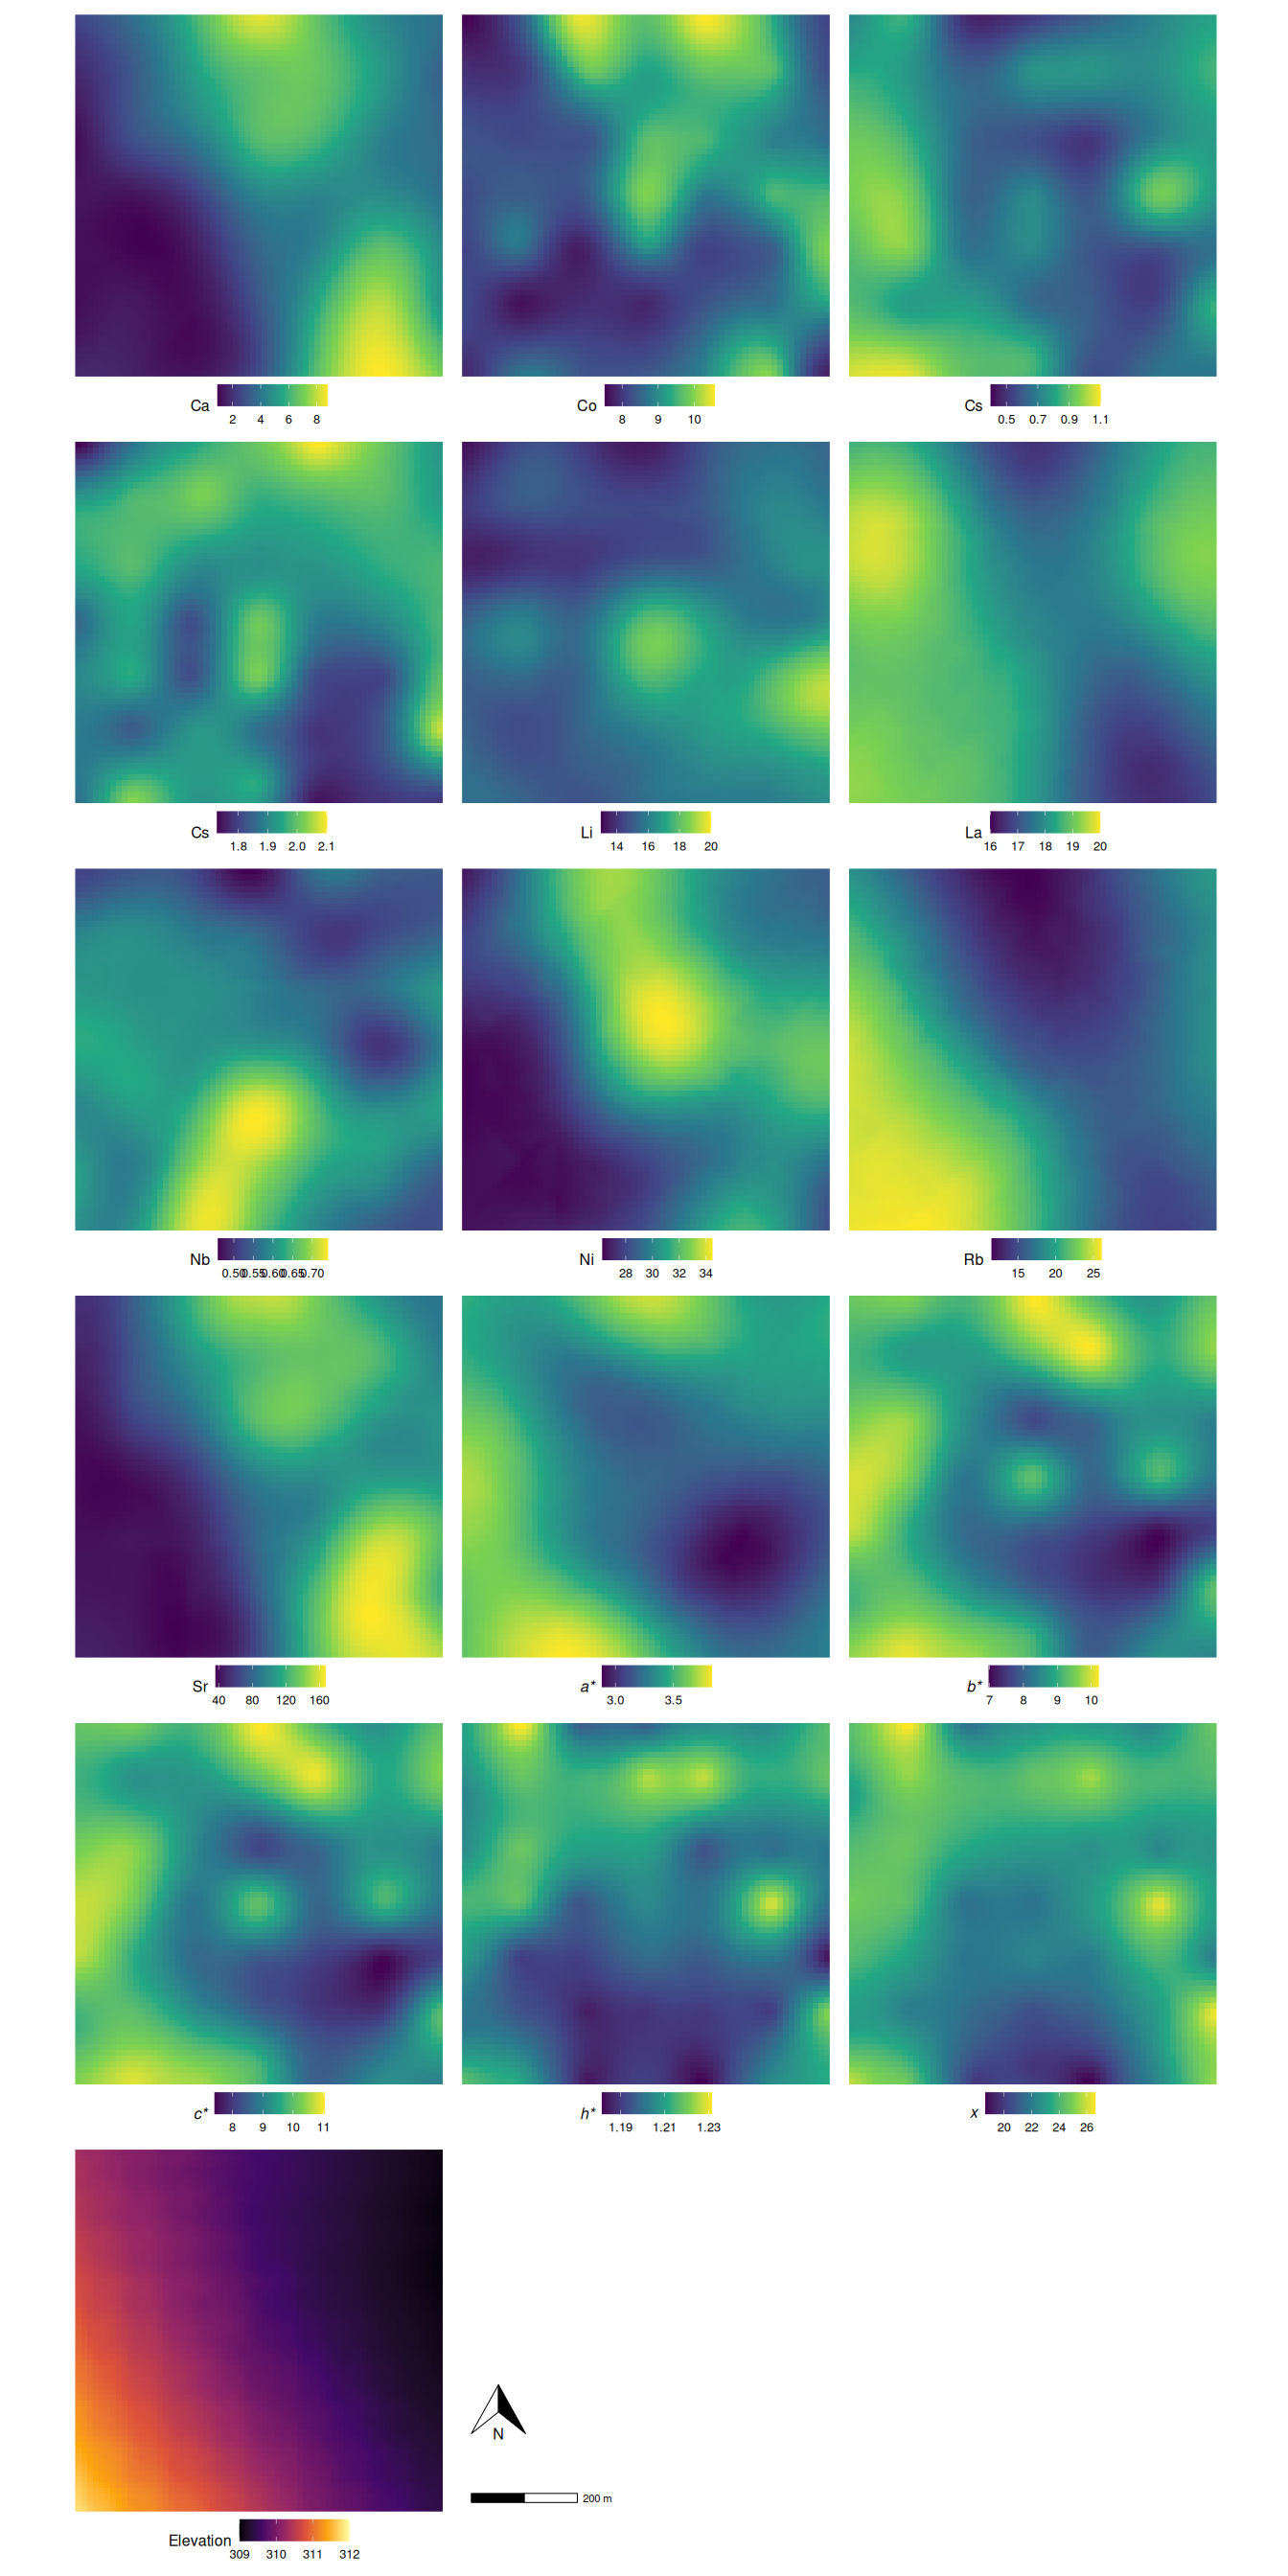
\includegraphics[keepaspectratio]{index_files/figure-latex/notebooks-property_maps-fig-ag_map-output-1.png}}

}

\caption{\label{fig-ag_map}Kriged maps of select colour and geochemical
properties and elevtion across the agricultural site.}

\end{figure}%

\textsubscript{Source:
\href{https://alex-koiter.github.io/spatial-variability-soil-manuscript/notebooks/property_maps.qmd.html\#cell-fig-ag_map}{Soil
property mapping}}

\begin{figure}[H]

\centering{

\pandocbounded{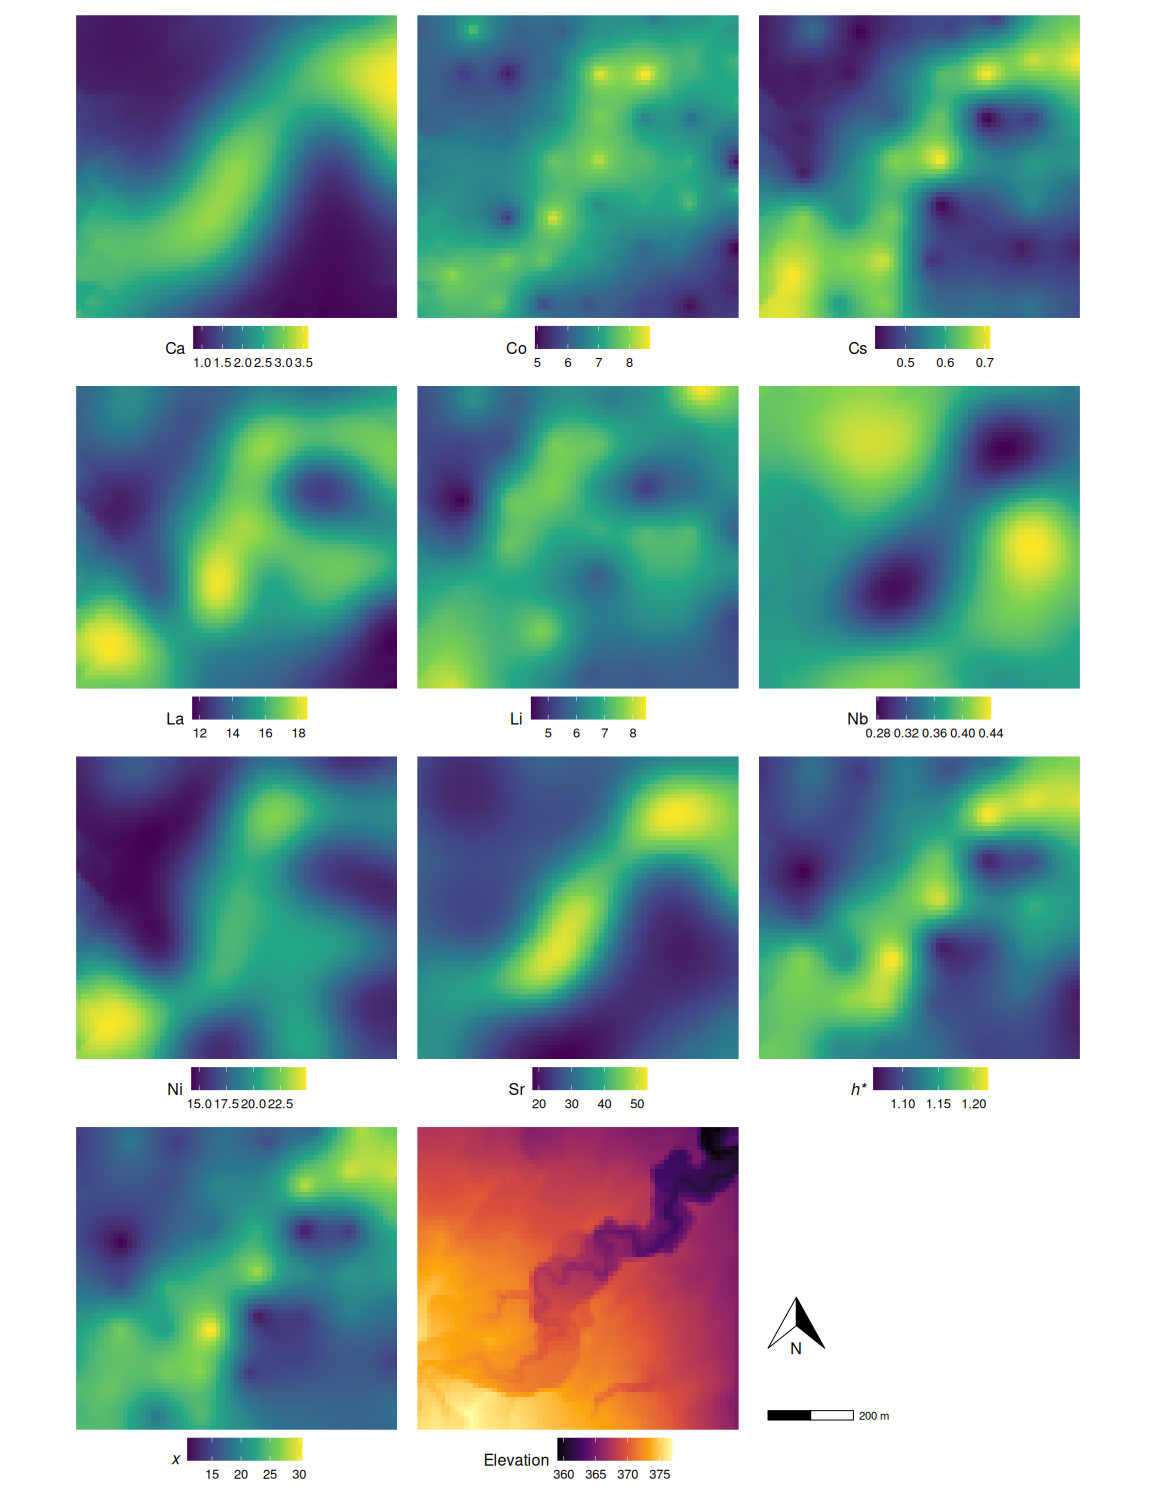
\includegraphics[keepaspectratio]{index_files/figure-latex/notebooks-property_maps-fig-forest_map-output-1.png}}

}

\caption{\label{fig-forest_map}Kriged map of select colour and
geochemical properties and elevation across the forested site.}

\end{figure}%

\textsubscript{Source:
\href{https://alex-koiter.github.io/spatial-variability-soil-manuscript/notebooks/property_maps.qmd.html\#cell-fig-forest_map}{Soil
property mapping}}

\begin{figure}[H]

\centering{

\pandocbounded{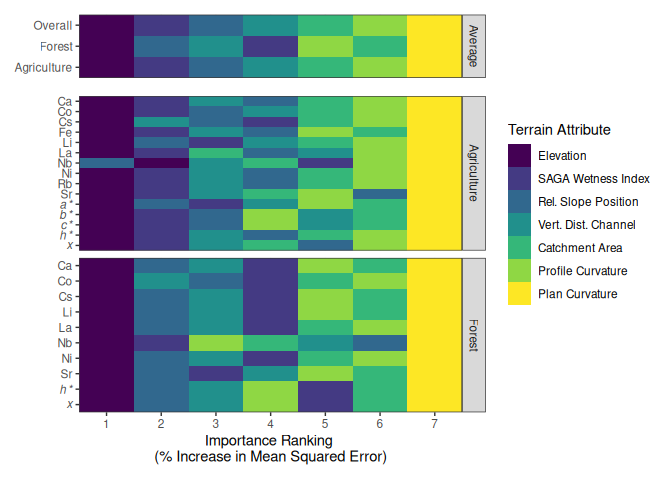
\includegraphics[keepaspectratio]{index_files/figure-latex/notebooks-RF_summary-fig-rf-results-output-1.png}}

}

\caption{\label{fig-rf-results}Heat map of the Random Forest regresssion
results showing the ranking of the importance of terrain attributes
(based on \% increase in Mean Squared Error) in explaining the spatial
variabilty of selected colour and geochemical properties within the
agricultural and forested sites. Top panel shows an average ranking for
each site and across both sites.}

\end{figure}%

\textsubscript{Source:
\href{https://alex-koiter.github.io/spatial-variability-soil-manuscript/notebooks/RF_summary.qmd.html\#cell-fig-RF-results}{Random
Forest summary}}

\begin{longtable}[]{@{}
  >{\centering\arraybackslash}p{(\linewidth - 10\tabcolsep) * \real{0.1667}}
  >{\centering\arraybackslash}p{(\linewidth - 10\tabcolsep) * \real{0.1667}}
  >{\centering\arraybackslash}p{(\linewidth - 10\tabcolsep) * \real{0.1667}}
  >{\centering\arraybackslash}p{(\linewidth - 10\tabcolsep) * \real{0.1667}}
  >{\centering\arraybackslash}p{(\linewidth - 10\tabcolsep) * \real{0.1667}}
  >{\centering\arraybackslash}p{(\linewidth - 10\tabcolsep) * \real{0.1667}}@{}}

\caption{\label{tbl-rf-summary}Model summary and performance statistics
for the random forest regression using the training, validation, and
test data sets.}

\tabularnewline

\toprule\noalign{}
\begin{minipage}[b]{\linewidth}\raggedright
Property
\end{minipage} & \begin{minipage}[b]{\linewidth}\raggedright
{MSETraining}{\textsuperscript{1}}
\end{minipage} & \begin{minipage}[b]{\linewidth}\raggedright
{}{\textsuperscript{2}}
\end{minipage} & \begin{minipage}[b]{\linewidth}\raggedright
{MSETesting}{\textsuperscript{1}}
\end{minipage} & \begin{minipage}[b]{\linewidth}\raggedright
{}{\textsuperscript{2}}
\end{minipage} & \begin{minipage}[b]{\linewidth}\raggedright
{\{\{R\^{}2\}\}Testing}
\end{minipage} \\
\midrule\noalign{}
\endhead
\midrule\noalign{}
\multicolumn{6}{@{}>{\centering\arraybackslash}p{(\linewidth - 10\tabcolsep) * \real{1.0000} + 10\tabcolsep}@{}}{%
{\textsuperscript{1}} Mean square error} \\
\multicolumn{6}{@{}>{\centering\arraybackslash}p{(\linewidth - 10\tabcolsep) * \real{1.0000} + 10\tabcolsep}@{}}{%
{\textsuperscript{2}} Percent variance explained} \\
\bottomrule\noalign{}
\endlastfoot
\multicolumn{6}{@{}>{\centering\arraybackslash}p{(\linewidth - 10\tabcolsep) * \real{1.0000} + 10\tabcolsep}@{}}{%
Agriculture} \\
Ca & 0.374 & 91.6 & 0.359 & 91.8 & 0.91 \\
Co & 0.089 & 79.8 & 0.080 & 82.5 & 0.80 \\
Cs & 0.002 & 85.7 & 0.002 & 86.4 & 0.85 \\
Fe & 0.001 & 69.6 & 0.001 & 70.9 & 0.69 \\
Li & 0.538 & 59.3 & 0.533 & 59.8 & 0.64 \\
La & 0.048 & 93.0 & 0.044 & 93.1 & 0.93 \\
Nb & 0.001 & 57.3 & 0.001 & 59.1 & 0.55 \\
Ni & 0.338 & 93.1 & 0.335 & 93.7 & 0.93 \\
Rb & 0.733 & 95.3 & 0.643 & 96.1 & 0.95 \\
Sr & 97.221 & 93.5 & 93.970 & 93.6 & 0.93 \\
a* & 0.007 & 85.0 & 0.006 & 86.9 & 0.85 \\
b* & 0.136 & 72.5 & 0.120 & 75.3 & 0.72 \\
c* & 0.155 & 73.2 & 0.136 & 75.9 & 0.73 \\
h* & 0.000 & 58.3 & 0.000 & 58.6 & 0.56 \\
x & 0.628 & 61.9 & 0.701 & 61.8 & 0.59 \\
\multicolumn{6}{@{}>{\centering\arraybackslash}p{(\linewidth - 10\tabcolsep) * \real{1.0000} + 10\tabcolsep}@{}}{%
Forest} \\
Ca & 0.231 & 61.1 & 0.231 & 60.7 & 0.63 \\
Co & 0.244 & 39.1 & 0.234 & 42.9 & 0.48 \\
Cs & 0.002 & 64.1 & 0.002 & 67.1 & 0.66 \\
Li & 0.278 & 41.3 & 0.282 & 42.0 & 0.46 \\
La & 1.401 & 43.3 & 1.323 & 47.5 & 0.48 \\
Nb & 0.001 & 55.0 & 0.001 & 55.9 & 0.58 \\
Ni & 2.819 & 55.2 & 2.806 & 56.0 & 0.55 \\
Sr & 29.427 & 59.4 & 29.663 & 59.1 & 0.59 \\
h* & 0.001 & 58.8 & 0.001 & 60.3 & 0.62 \\
x & 5.646 & 62.6 & 5.810 & 63.4 & 0.64 \\

\end{longtable}

\textsubscript{Source:
\href{https://alex-koiter.github.io/spatial-variability-soil-manuscript/notebooks/RF_summary.qmd.html\#cell-tbl-RF-summary}{Random
Forest summary}}

\section*{References}\label{references}
\addcontentsline{toc}{section}{References}

\renewcommand{\bibsection}{}
\bibliography{references.bib}

\section*{Supplemental figures}\label{supplemental-figures}
\addcontentsline{toc}{section}{Supplemental figures}

\begin{suppfig}

\centering{

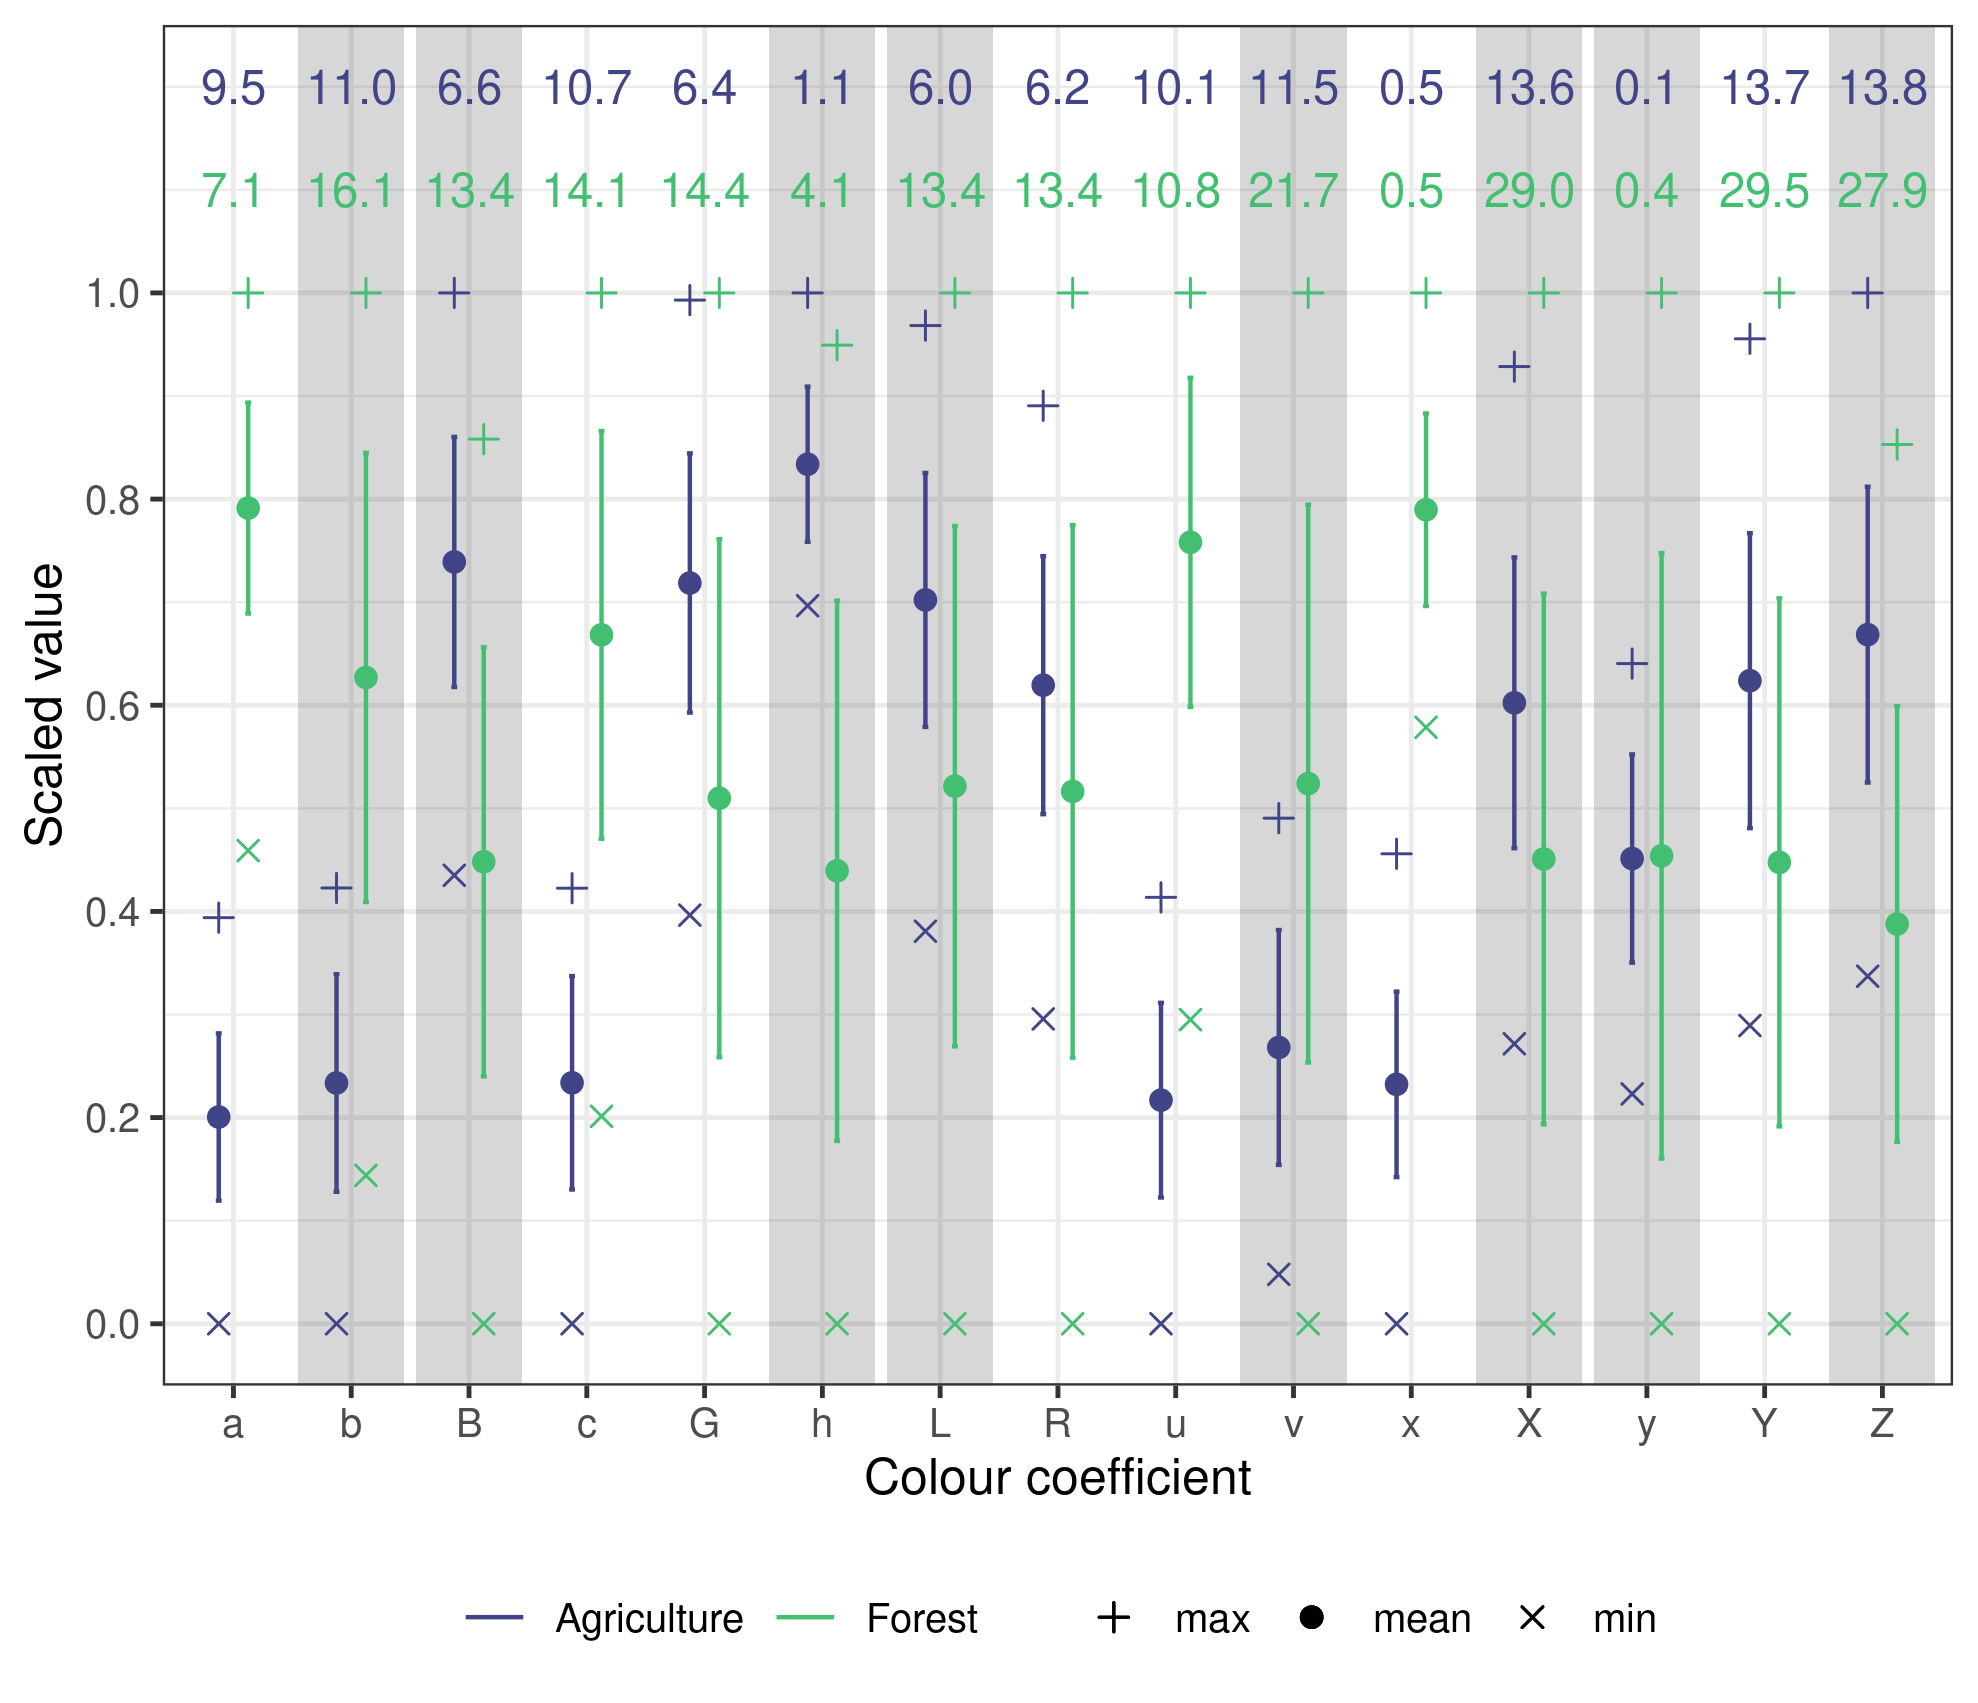
\includegraphics[width=1\linewidth,height=\textheight,keepaspectratio]{images/colour_summary.png}

}

\caption{\label{suppfig-colour_summary}Summary statistics of all
measured colour soil properties at both sites. Error bars represent 1SD
and the numeric values indicate the CV.}

\end{suppfig}%

\begin{suppfig}

\centering{

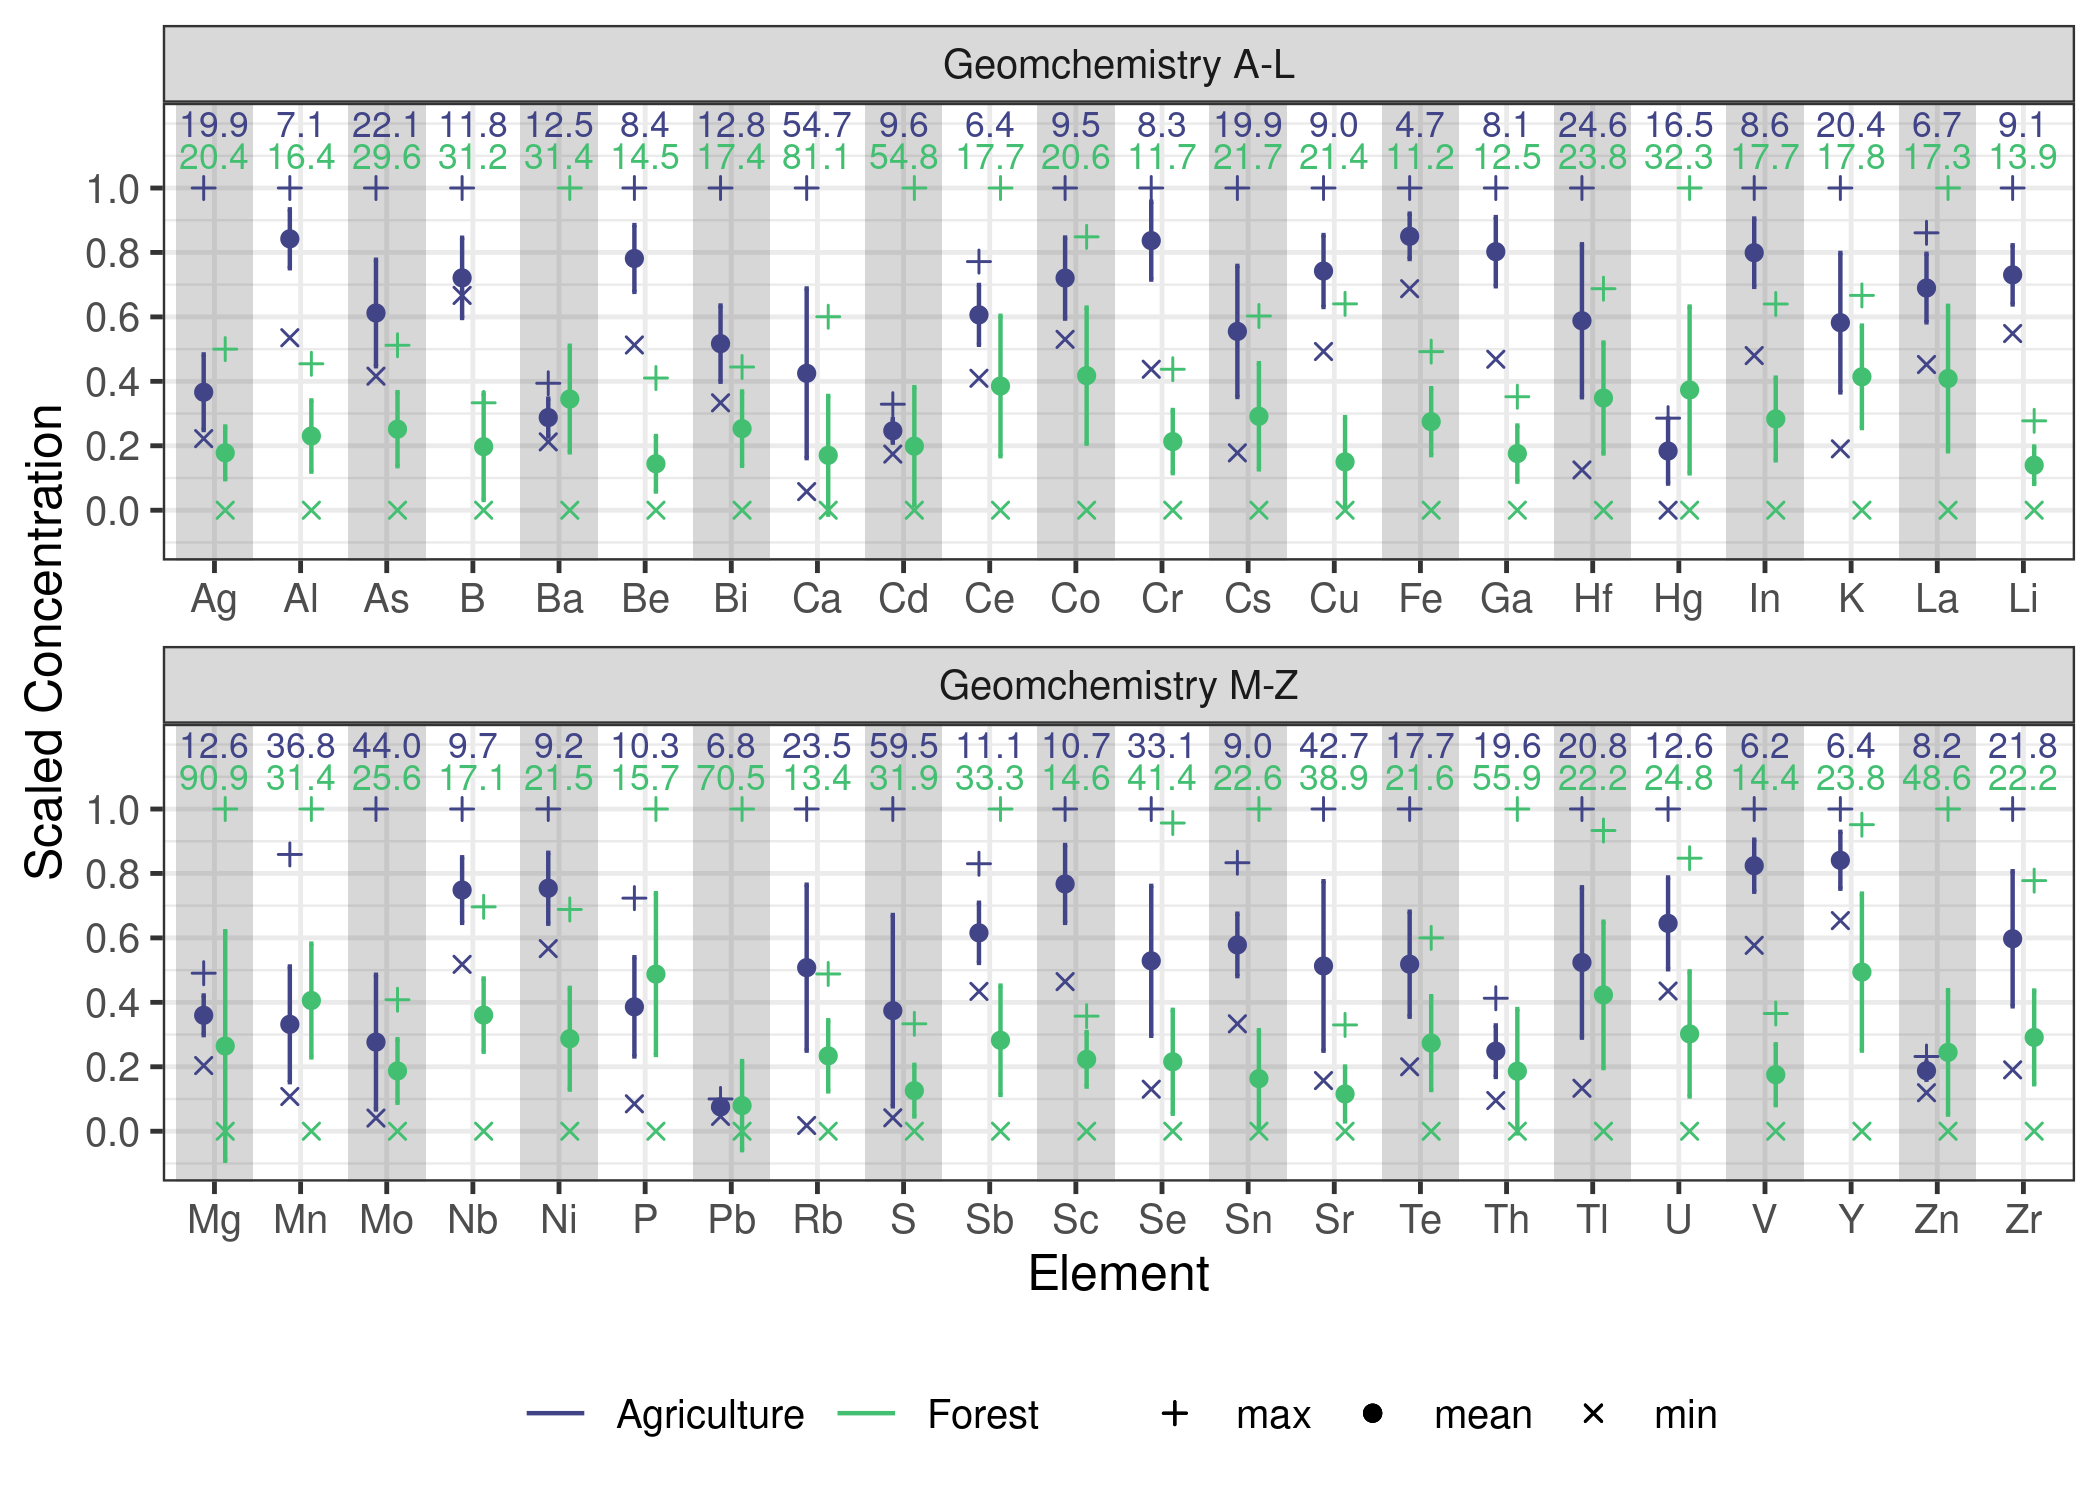
\includegraphics[width=1\linewidth,height=\textheight,keepaspectratio]{images/geo_summary.png}

}

\caption{\label{suppfig-geo_summary}Summary statistics of all measured
geochemical soil properties at both sites. Error bars represent 1SD and
the numeric values indicate the CV.}

\end{suppfig}%

\section*{Supplemental tables}\label{supplemental-tables}
\addcontentsline{toc}{section}{Supplemental tables}

\begin{supptab}

\caption{\label{supptab-abbrev}Description of spectral reflectance
colour coefficients used as fingerprints. Reproduced from Boudreault et
al.~(2018)}

\centering{

\begin{longtable*}[]{@{}
  >{\raggedright\arraybackslash}p{(\linewidth - 4\tabcolsep) * \real{0.2917}}
  >{\raggedright\arraybackslash}p{(\linewidth - 4\tabcolsep) * \real{0.4583}}
  >{\raggedright\arraybackslash}p{(\linewidth - 4\tabcolsep) * \real{0.2500}}@{}}
\toprule\noalign{}
\begin{minipage}[b]{\linewidth}\raggedright
\textbf{Colour space model}
\end{minipage} & \begin{minipage}[b]{\linewidth}\raggedright
Parameter
\end{minipage} & \begin{minipage}[b]{\linewidth}\raggedright
Abbreviation
\end{minipage} \\
\midrule\noalign{}
\endhead
\bottomrule\noalign{}
\endlastfoot
RGB & Red & R \\
RGB & Green & G \\
RGB & Blue & B \\
CIE xyY & Chromatic Coordinate x & x \\
CIE xyY & Chromatic Coordinate y & y \\
CIE xyY & Brightness & Y \\
CIE XYZ & Virtual component X & X \\
CIE XYZ & Virtual component Z & Z \\
CIE LAB & Metric lightness function & L \\
CIE LAB & Chromatic coordinate opponent red--green scales & \emph{a*} \\
CIE LAB & Chromatic coordinate opponent red--green scales & \emph{b*} \\
CIE LUV & Chromatic coordinate opponent blue--yellow scales &
\emph{u*} \\
CIE LUV & Chromatic oordinate opponent red--green scales & \emph{v*} \\
CIE LCH & CIE hue & \emph{c*} \\
CIE LCH & CIE chroma & \emph{h*} \\
\end{longtable*}

}

\end{supptab}%

\begin{supptab}

\caption{\label{supptab-correlation2}Pearson's correlation coefficients
for soil properties and terrain attributes using interpolated values
(10m resolution).}

\centering{

\begin{table}
\fontsize{12.0pt}{14.4pt}\selectfont
\begin{tabular*}{\linewidth}{@{\extracolsep{\fill}}llrlrlll}
\toprule
Property & Elevation & SAGA Wetness Index & Rel. Slope Position & Vert. Dist. Channel & Catchment Area & Plan Curvature & Profile Curvature \\ 
\midrule\addlinespace[2.5pt]
\multicolumn{8}{l}{{\bfseries Agriculture}} \\[2.5pt] 
\midrule\addlinespace[2.5pt]
Ca & -0.76*** & 0.59*** & -0.26*** & -0.25*** & 0.1*** & NS & NS \\ 
Co & -0.63*** & 0.61*** & -0.23*** & -0.24*** & 0.14*** & NS & NS \\ 
Cs & 0.58*** & -0.45*** & 0.06*** & 0.14*** & -0.11*** & NS & NS \\ 
Fe & -0.14*** & 0.32*** & -0.09*** & -0.09*** & 0.09*** & NS & NS \\ 
Li & -0.4*** & 0.27*** & -0.42*** & -0.2*** & 0.13*** & NS & NS \\ 
La & 0.53*** & -0.3*** & 0.07*** & 0.15*** & NS & NS & NS \\ 
Nb & 0.48*** & -0.52*** & 0.25*** & 0.15*** & -0.08*** & NS & NS \\ 
Ni & -0.75*** & 0.71*** & -0.32*** & -0.32*** & 0.2*** & NS & NS \\ 
Rb & 0.81*** & -0.71*** & 0.24*** & 0.3*** & -0.15*** & NS & NS \\ 
Sr & -0.81*** & 0.64*** & -0.35*** & -0.27*** & 0.12*** & NS & NS \\ 
\emph{a}* & 0.61*** & -0.44*** & 0.35*** & 0.23*** & -0.12*** & NS & NS \\ 
\emph{b}* & 0.39*** & -0.22*** & 0.22*** & 0.1*** & -0.09*** & NS & NS \\ 
\emph{c}* & 0.41*** & -0.24*** & 0.22*** & 0.11*** & -0.09*** & NS & NS \\ 
\emph{h}* & -0.22*** & 0.31*** & -0.15*** & -0.15*** & NS & NS & NS \\ 
\emph{x} & -0.15*** & 0.25*** & -0.23*** & -0.12*** & NS & NS & NS \\ 
\midrule\addlinespace[2.5pt]
\multicolumn{8}{l}{{\bfseries Forest}} \\[2.5pt] 
\midrule\addlinespace[2.5pt]
Ca & -0.11*** & -0.47*** & 0.09*** & 0.4*** & 0.24*** & 0.1*** & NS \\ 
Co & -0.04* & -0.34*** & 0.05*** & 0.32*** & 0.15*** & 0.05** & -0.03* \\ 
Cs & 0.09*** & -0.4*** & 0.17*** & 0.34*** & 0.18*** & 0.06*** & -0.03* \\ 
Li & 0.1*** & -0.15*** & 0.05*** & 0.18*** & 0.07*** & NS & NS \\ 
La & NS & -0.23*** & NS & 0.24*** & 0.11*** & 0.05*** & NS \\ 
Nb & 0.12*** & 0.46*** & -0.11*** & -0.34*** & -0.21*** & -0.09*** & 0.05*** \\ 
Ni & 0.19*** & -0.27*** & 0.14*** & 0.2*** & 0.04** & NS & NS \\ 
Sr & -0.34*** & -0.44*** & -0.12*** & 0.36*** & 0.26*** & 0.11*** & -0.05** \\ 
\emph{h}* & -0.08*** & -0.36*** & NS & 0.35*** & 0.22*** & 0.08*** & -0.03* \\ 
\emph{x} & -0.04** & -0.38*** & 0.09*** & 0.35*** & 0.22*** & 0.09*** & -0.03* \\ 
\bottomrule
\end{tabular*}
\begin{minipage}{\linewidth}
*** p < 0.001; ** p < 0.01; * p < 0.05; NS = non-significant at p = 0.05\\
\end{minipage}
\end{table}

\textsubscript{Source:
\href{https://alex-koiter.github.io/spatial-variability-soil-manuscript/index.qmd.html}{Article
Notebook}}

}

\end{supptab}%





\end{document}
